\chapter{The Vernier Analysis}
\label{ch:vernier_analysis}
\section{Overview}

The Vernier Scan Analysis is typically done every year, its purpose is to
calculate the absolute luminosity of collisions delivered to PHENIX's
interaction region (IR) by RHIC.  Absolute luminosity is a necessary for the
normalization of any cross-section. This chapter describes the process of
carrying out the vernier analysis for the 2012 data set, but it was also
carried out for the 2013 data set.

A vernier scan describes the process where, in a controlled manner, one beam is
scanned across another beam, and held at fixed positions. The purpose of this
maneuver is to enable direct measurement of the transverse profile of the blue
and yellow beam (assumed to be identical). The scanning serves a second purpose,
in that, if one observes the distribution of event collision vertex (in z), the
shape of the distribution provides information about the value of the beam
focusing parameter $\beta^*$, and the crossing angle between the beams.

Measuring the transverse beam profile allows on to calculate from first
principals the expected machine luminosity delivered to PHENIX,
$\mathcal{L}_{RHIC}$. This luminosity is corrected for both the beam focusing
effect, and the crossing angle. Neglecting to correct both effects leads to
about a 10\% reduction in measured luminosity. 

The vernier scan also provides an opportunity to calculate the efficiency of the
minimum bias BBC novertex trigger, which enables the BBCs to be used as a
luminosity monitor for physics operations. 

For the BBC trigger, we can represent, the relationship between $\mathcal{L}$
and the cross section observed by the BBC as:

\begin{equation} 
\label{eq:lumi_xsec_simple} 
\mathcal{L}_{BBC} = {R_{BBC}\over\sigma_{BBC}} 
\end{equation}

{\noindent}Where $\mathcal{L}_{BBC}$ is the effective luminosity delivered to a
specific BBC trigger, $R_{BBC}$ is the live event rate of the BBC trigger, and
$\sigma_{BBC}$ is defined as the cumulative cross section of events measured by
this trigger.

{\noindent}The absolute luminosity is calculated as:

\begin{equation} 
\label{eq:lumi_one_bunch} 
\mathcal{L} = {f_{bunch}N_{b} N_{y}\over{2\pi\sigma_{x}\sigma_{y}}} 
\end{equation}

Where $\mathcal{L}$ is the absolute luminosity, $f_{bunch}$ is the frequency of
each individual bunch crossing, $N_{b}, N_{y}$ are the bunch populations for the
specific blue and yellow beams, respectively, and $\sigma_{x}, \sigma_{y}$ are
the transverse widths of both bunches in the $x$ and $y$ directions (see the
PHENIX coordinate system for more details on the origin of these measurements,
Figure~\ref{fig:phenix_coordinate_system}). We assume identical beam bunch
distributions for the blue and yellow beams~\cite{AN888Datta2010}.

Filled bunches cross once every beam clock tick. Therefore, for $120$ bunch
fills (including filled and empty bunches), and the standard blue beam clock
frequency, $f_{clock}$, of $9.36 MHz$, $f_{bunch} \equiv f_{clock} / 120 = 78
kHz$.

This work builds upon previous Vernier Analyses undertaken at PHENIX,
\cite{AN184Belikov2003}, \cite{an597Bazilevsky2007}, \cite{an688Bennett2008},
\cite{AN888Datta2010}, and \cite{Drees2009}.

Global vernier scan characteristics are summarized in table
~\ref{tab:global_scan_summary}. Each vernier scan is done slightly differently
as a systematic check - beam scan order is varied, beam energy is varied, scan
length and step length is varied, and scanning patterns are varied. These
variations are not expected to produce changes in the final luminosity
calculation.

\begin{sidewaystable}[ht]
\centering
\begin{tabular}{ccccccccc}
\toprule
\textbf{Run}    & \textbf{Fill}   & \textbf{Energy}          & \textbf{Scan}       & \textbf{Scan}    & \textbf{Scan}  & \textbf{Beam}    &                & \textbf{Step}     \\
\textbf{Number} & \textbf{Number} & \textbf{($GeV\sqrt{s}$)} & \textbf{Time (min)} & \textbf{Pattern} & \textbf{Order} & \textbf{Scanned} & \textbf{Steps} & \textbf{Time (s)} \\
\midrule
359711 & 16444 & 200 & 41 & Type 1 & H - V & Blue  & 26 & 57.5 \\
360879 & 16470 & 200 & 41 & Type 1 & H - V & Yellow& 26 & 61.2 \\
362492 & 16514 & 200 & 50 & Type 1 & V - H & Blue  & 26 & 62.3 \\
364636 & 16587 & 510 & 58 & Type 2 & H - V & Yellow& 18 & 21.7 \\
365866 & 16625 & 510 & 53 & Type 1 & H - V & Blue  & 26 & 70.0 \\
366605 & 16655 & 510 & 54 & Type 1 & H - V & Yellow& 26 & 67.7 \\
367138 & 16671 & 510 & 54 & Type 1 & H - V & Blue  & 26 & 68.65\\
\bottomrule
\end{tabular}
\caption{ A summary of vernier scans in run 12 }
\label{tab:global_scan_summary}
\end{sidewaystable}

Two different scanning patterns were used in Run 12, summarized in
Figure~\ref{fig:scan_patterns}. Scan Type 2 was previously used in past years
prior to 2012, and is included in this year's set of scans as a consistency
check. Type 2 scanning describes the pattern where beams begin maximally
overlapped, and are gradually displaced to maximum displacement, brought into
maximum overlap again, then gradually displaced in the opposite direction.
Type 1 was used for the majority of the scans in 2012, and consists of beams
begining maximally overlapped, then maximally displaced, and swept back through
maximum overlap, continuing, and ending maximally displaced. The scan order
does not effect the final luminosity, provided that beam losses are properly
accounted for.

\begin{figure}[ht] 
  \centering
  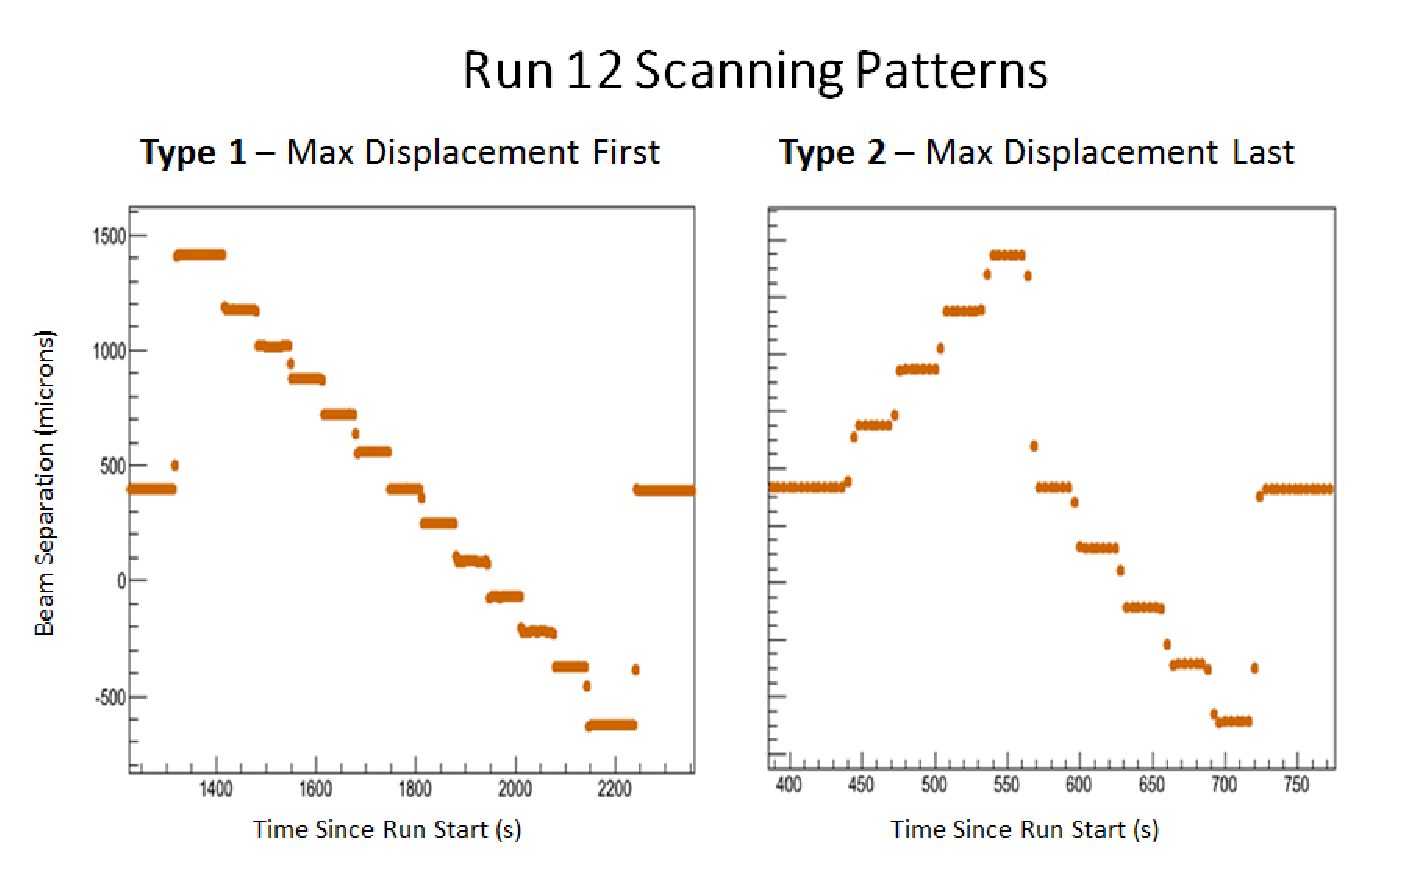
\includegraphics[width=0.75\linewidth]{./figures/scan_patterns} 
  \caption{ 
    Left Panel: Type 1 scanning pattern. Right Panel: Type 2 scanning pattern.
    In both panels, we see the mean beam displacement as a function of time
    since the beginning of the vernier scan.
  }
  \label{fig:scan_patterns}
\end{figure}

\section{Variables and Calculations}
\label{sec:VariablesAndCalculations}

Variables used in the Vernier Analysis are chosen because they characterize the
dynamics of the beams intersecting in the PHENIX interaction region (IR). The
goal in the vernier analysis is to calculate the effective detector cross
section for our Beam Beam Counter, as well as the RHIC machine luminosity,
$\mathcal{L}_{RHIC}$. We must also use a realistic model for highly relativistic
collisions between two intersecting beams.

The basic equations, models and variables used in the analysis are summarized
here. I will go into detail discussing the extraction of each parameter within
relevant section.

The effective detector cross section~\cite{Drees2013} can be expressed as:

\begin{equation}
\label{eq:detector_xsec}
\sigma_{ZDC}^{eff} = {{R_{max} 2\pi n_{B} n_{Y} \sigma_{x} \sigma_{y}}\over{n_{bunch}
f_{bunch} N_{B} N_{Y} }}
\end{equation}

{\noindent}with various parameters are defined in Table~\ref{tab:ana_vars}.

{\noindent}We use the standard relativistic intersecting beam model for
colliding bunches~\cite{an888}, which is defined to be:

\begin{equation}
\label{eq:reletivistic_beam_final} 
\mathcal{L} = {{n_{bunch} f_{bunch} N_{B} N_{Y} }\over{ 2 \pi^{2} \sigma_{x}
\sigma_{y}\sigma{z}^2}} \int \int
e^{-\left({{z^{2}}\over{\sigma_{z}^{2}}}+{{c^{2}t^{2}}\over{\sigma_{z}^{2}}}\right)} c dt
\end{equation}

The full summary of the variables either extracted or directly used in this
analysis are presented in Table~\ref{tab:ana_vars}.

\begin{table}[ht]
  \centering
  \begin{tabular}{c p{8cm} c c }
    \toprule
    \textbf{Variable} & \textbf{Description} & \textbf{Units} & \textbf{Dimension} \\
    \midrule 
    $\sigma_{x}$, $\sigma_{y}$ & bunch profile width obtained from vernier scan beam overlap in x and y directions. & $\mu m$ & $length$ \\
    $\sigma_{z}$ & bunch profile width in z-direction, i.e. z-beam width. & $\mu m$ & $length$ \\
    $\dot{N}$ & Live event rate for "BBCLL1(\textgreater0 tubes)" trigger & $Hz$ & $time^{-1}$ \\
    $R_{max}$ & Maximum BBC Rate determined from maximum overlap of beams rate for "BBCLL1(\textgreater0 tubes)" trigger & $Hz$ & $time^{-1}$ \\
    $\mathcal{L}_{RHIC}$ & Absolute luminosity delivered to PHENIX IR from RHIC & $cm^{-2}s^{-1}$ & $area^{-1}time^{1}$ \\
    $\sigma_{p+p} $ & Inelastic scattering cross section of proton-proton collisions & $cm^{2}$ & $area^{-1}$ \\
    $N_{b}^{i},N_{y}^{i}$ & Number of ions in bunch $i$ for the blue ($b$) beam or yellow ($y$) beam. & count & \\
    $f_{bunch}$ & Frequency of a specific bunch crossing & $Hz$ & $seconds^{-1}$ \\
    $k_{b}$ & Number of bunches filled in one of the beams (assume identical beams) & count & \\
    $\sigma_{BBC}$ & Cross section of p+p collisions observed by BBC,
    uncorrected for efficiency & $cm^{-2}$ & $area^{-1}$ \\
    $\epsilon_{BBC}$ & BBC efficiency & unitless $[0,1]$ & \\
    $n_{bunch}$ & Number of filled bunches in the blue or yellow beam & unitless $[0,120]$ & \\
    \bottomrule
  \end{tabular}
  \caption{
    The variables we use in the vernier analysis. Some variables are extracted
    directly from the data streams (such as the bbc-rate), while others are
    calculated from distributions of variables (such as the beam-width,
    $\sigma_{x,y}$). 
  }
  \label{tab:ana_vars}
\end{table}

\section{Data Streams}
\label{ch:DataStreams}

PHENIX software and the overall DAQ structure was discussed in
Chapter~\ref{ch:experimental_apparatus}. The vernier analysis is only interested
in understanding the frequency of minimum bias events, one does not do any
physical event reconstruction beyond determining the event $z$-vertex. To
characterize the vernier scan, the following data streams are used:

\begin{itemize}
\item PRDF Data (available on either 1 second intervals, or event-by-event basis)
  \begin{itemize}
  \item GL1P-0: "BBCLL1(\textgreater0 tubes)"
  \item GL1P-1: "CLOCK"
  \item GL1P-2: "ZDCLL1Wide"
  \item GL1P-3: "ZDCLL1Narrow"
  \item event-sequence
  \item ATP number
  \item epoch time stamp
  \item GL1 crossing ID (bunch number)
  \end{itemize}
\item BPM Data (available in four second intervals)
  \begin{itemize}
  \item Sector 7 Blue Beam x position
  \item Sector 7 Blue Beam y position
  \item Sector 7 Yellow Beam x position
  \item Sector 7 Yellow Beam y position
  \item Sector 8 Blue Beam x position
  \item Sector 8 Blue Beam y position
  \item Sector 8 Yellow Beam x position
  \item Sector 8 Yellow Beam y position
  \item epoch time stamp
  \end{itemize}
\item WCM and DCCT Data (avaialble every few seconds)
  \begin{itemize}
  \item WCM population for each bunch
  \item DCCT beam current for blue beam
  \item DCCT beam current for yellow beam
  \item epoch time stamp associated with each field of WCM or DCCT data
  \end{itemize}
\item DST Data
  \begin{itemize}
  \item BbcOut Node
    \begin{itemize}
      \item BBC pmt tubes fired north
      \item BBC pmt tubes fired south
      \item BBC event z-vertex
    \end{itemize}
  \end{itemize}
  \begin{itemize}
  \item ZdcOut Node
    \begin{itemize}
      \item ZDC event z-vertex
    \end{itemize}
  \end{itemize}
  \begin{itemize}
  \item TrigLvl1 Node
    \begin{itemize}
      \item bitmasked triglive
      \item bitmasked trigscaled
      \item bitmasked trigraw
    \end{itemize}
  \end{itemize}  
  \begin{itemize}
  \item SpinDataEventOut Node
    \begin{itemize}
      \item GL1P crossing ID
      \item event-sequence
      \item GL1P-0: "BBCLL1(\textgreater0 tubes)"
      \item GL1P-1: "CLOCK"
      \item GL1P-2: "ZDCLL1Wide"
      \item GL1P-3: "ZDCLL1Narrow"
    \end{itemize}
  \end{itemize}  
\end{itemize}

The vernier analysis is unique among various PHENIX analyses because it requires
that data streams from RHIC machine sources and the PHENIX detector are
synchronized. It is also unique in that the data set itself exhibits obvious time
dependent behavior. This introduces interesting challenges, as PHENIX software
generally does not provide tools to deal with time dependent data, and
synchronization of PHENIX data with other RHIC data streams is infrequently
done. PHENIX and RHIC data streams effectively live in entirely different
software universes (post data production), so there is no guarantee of a common
key which can be used to synchronize the data. 

Previous analyses have generally dealt with each data stream separately,
combining only when absolutely necessary. This approach favors simplicity, but
is generally hard to generalize to any data set from any year. PHENIX data sets
are analyzed as a phase-space data set, with no desire to understand or account
for time dependent effects.  However, the vernier analysis is intrinsically a
time-dependent analysis, so it makes intuitive sense to do the analysis in a way
which mirrors the physical process of the vernier scan. This means that for
portions of the analysis, one must resort to using raw PHENIX data, which
requires a small amount of custom software to be written.

By understanding the data structures which are available, I have written
software which can generally cross check and reproduce any vernier analysis that
has been undertaken in previous years, and this has been exploited to provide
fast cross-checks for other years' vernier analyses. The Common-Device (CDEV)
data packet contained in PHENIX Raw Data Format files contains timing
information needed to synchronize the detector data, with the data from RHIC. 

\section{Beam Position Monitors}
There are two beam position monitors BPM(s) located about 8 meters away from the
PHENIX IR on either side (BPM sector 7, and BPM sector 8). The BPMs may be used
to establish the relative separation of the blue and yellow beams, but are not
good for establishing absolute beam position~\cite{Drees2013}.  

The BPM data obtained contains measurements of beam position over the course of
an entire fill. The start and end run times recorded in the PHENIX run data
base are used to isolate a chunk of BPM data corresponding to the vernier scan
using epoch time. The BPM data set contains the following fields:
\begin{itemize}
\item epoch time
\item blue beam, sector 7 $x$ position
\item blue beam, sector 7 $x$ position
\item blue beam, sector 8 $y$ position
\item blue beam, sector 8 $y$ position
\item yellow beam, sector 7 $x$ position
\item yellow beam, sector 7 $x$ position
\item yellow beam, sector 8 $y$ position
\item yellow beam, sector 8 $y$ position
\end{itemize}

The beam position monitors are coupled capacitively to the beam
pipe(Figure~\ref{fig:bpm_schematic_cartoon}), with pick ups on the left and
right of the pipe, and pickups above and below the pipe. Every four seconds,
data is read out from the BPMs. 

The method of BPM transduction of beam current to transverse beam position is
described in Figure~\ref{fig:bpm_schematic_cartoon}. The beam current, passing
through the BPM,  induces a time dependent voltage proportional to the
derivative of the beam current itself. BPM electronics use a comparator circuit,
and the readings from pickups situated around the beam pipe are used to
determine the $x$ and $y$ beam positions. The absolute measurement of beam
position is subject to offsets stemming from various effects, but the relative
beam displacement is reliable~\cite{kawallfocus2005}


The data stream provides an $x$ and $y$ position, plus an epoch time stamp
associated with the blue and yellow beams, from sector 7 and sector 8 BPMs.
With this data, one can geometrically extrapolate the intersection of the blue
and yellow beams respectively in the PHENIX IR plane, and then calculate the
net separation between the two beams, Figure ~\ref{fig:bpm_ir_xing_cartoon}.
Three parallel planes are defined, each plane perpendicular to the beam axis.
One places the planes at Sector 7 BPM location, the PHENIX IR, and Sector 8 BPM
location.  The two BPM planes are equidistant from the PHENIX IR. One can
geometrically solve for the equation for the line, given intersections at the
BPM Sector 7 plane, and the BPM Sector 8 plane, and extrapolate the beams'
intersection with the IR plane. From this intersection, one obtains the net
beam displacement.


\begin{figure}[ht]
  \begin{center}
    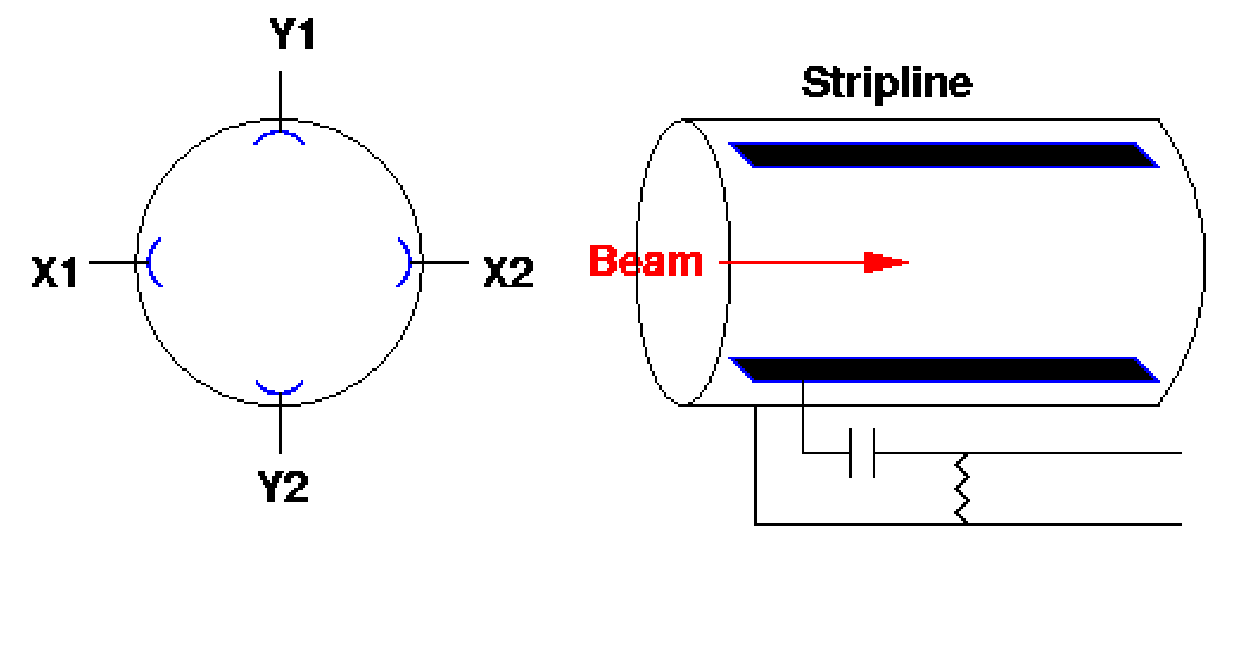
\includegraphics[width=1.0\linewidth]{./figures/bpm_schematic}
    \caption{ 
      BPM electronics use a comparator circuit, and the readings from X1/2 and
      Y1/2 to determine the $x$ and $y$ beam positions. 
    }
    \label{fig:bpm_schematic_cartoon}
  \end{center}
\end{figure}


\begin{figure}[ht]
\begin{center}
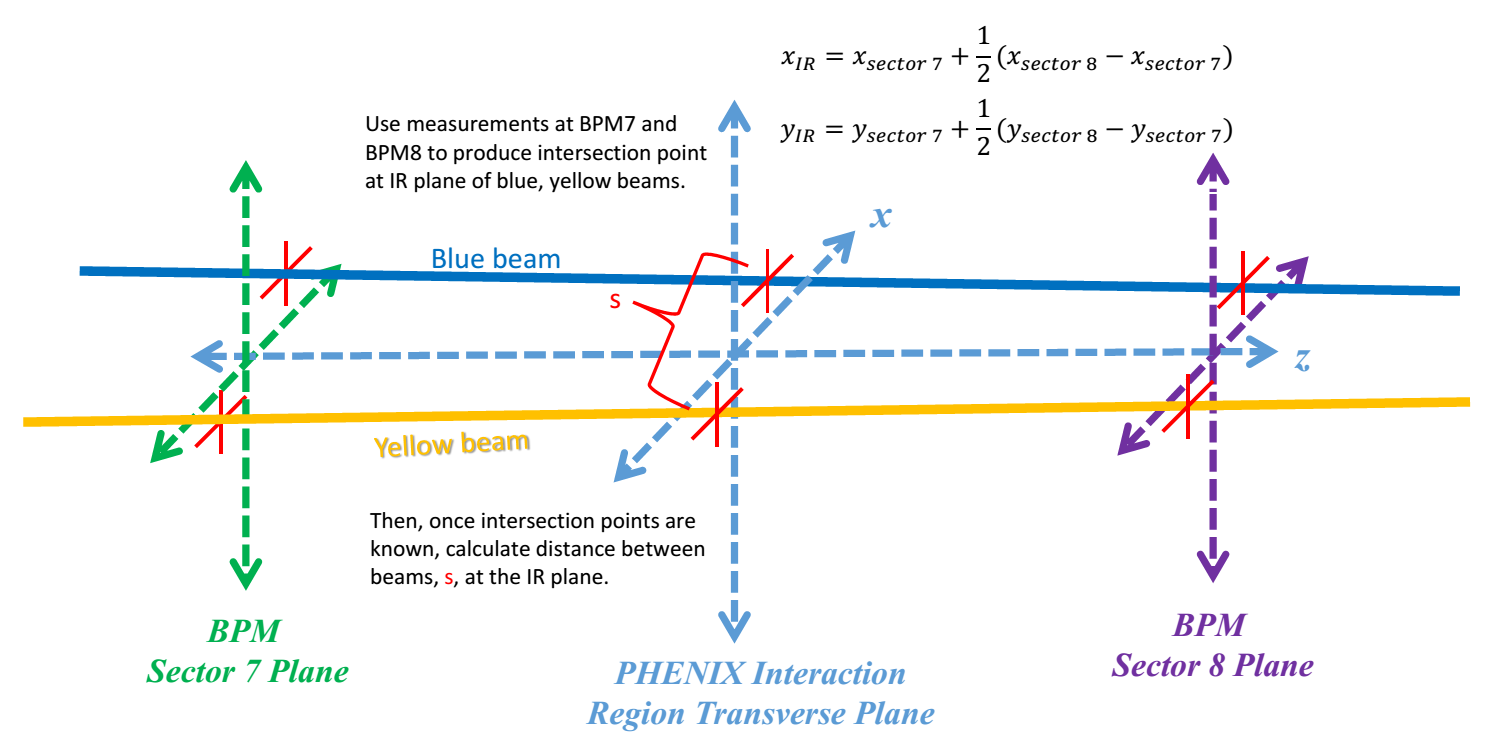
\includegraphics[width=1.0\linewidth]{./figures/bpm_ir_beam_separation}
\caption{
  Shown: the geometric extrapolation of beam displacement at the IR plane.
}
\label{fig:bpm_ir_xing_cartoon}
\end{center}
\end{figure}

\section{PHENIX Raw Data Format} 

The PHENIX raw data format (better known as PRDFs) are the form that recorded
data takes immediately after being assembled into events, by the PHENIX DAQ.
PRDF data is archived soon after being generated on the massive robotic tape
file-system. PRDF data is hierarchical. It is first organized by event-type,
and then organized by packet-type.  Every packet has a header, which contains
general information such as what the packet contains, and in what order that
packet was received from the DAQ. Every packet recorded can be associated with
a unique event-sequence number, which specifies roughly the order in which the
event owning the packet was received by the DAQ. Within a given run number, an
event-number is guaranteed to be unique. The complexity of the packet is
limited by the bandwidth available to move data off PHENIX onto other storage,
and the buffers/reconstruction ability of the front end electronics modules
built onto PHENIX subsystems.

Generally, raw PHENIX data is too complex to use straight-away, because minimal
to no reconstruction of physical properties for a certain event is done (and
this varies by the subsystem, and hardware constraints of the subsystem).
However, for the vernier analysis, we are generally only interested in very,
very simple properties of an event, all of which are completely available
directly from the PRDF. This allows us a huge flexibility, as other then the
libraries required to dump packet information from PRDFs headers, there are no
dependencies for obtaining the data we need from PRDFs.

One constraint of using PRDFs as a primary data source is disk space. A normal
physics run may be segmented into hundreds of PRDFs, each at 20 GB in size.
However, because the event rates are on average quite low for a vernier scan,
and because vernier scans typically do not last longer than 20 minutes, there
are typically only five or six PRDFs needed to store an entire scan. The data extracted from PRDFs is summarized in table~\ref{tab:prdf_data_summary}.

\subsection{GL1-1P Scalers, ATP Numberand Event Time Stamps}

The DAQ supports 32 possible triggers, which may be designed to be arbitrarily
sensitive to arbitrary hardware signal coincidences (see
Section~\ref{sec:triggering_aquisition}). When PHENIX experiences a trigger,
all PHENIX detector subsystems dump the FEM buffers to the sub-event builders
(SEB) which reconstruct raw events, and then pass these events along to the
ATPs (Assembly and Trigger Processor) to compress and assemble the events into
PRDFs. Over the course of this process, the event is categorized by event type.
For this analysis, we consider ``DATAEVENT'' event types and ``SCALEREVENT''
event types. There are 64 ATPs in total, and each ATP tags the event it
recieved with an ATP number $0 \leq ATPNUMBER < 64$, corresponding to the ATP
which processed the event and given an epoch time-stamp. 

Since time is synchronized between the ATPs via the network, there may be some
latency, and these time stamps must be corrected for an offset.  Because of the
large volume of data, several thousand events will arrive for processing
simultaneously, so one can simply choose an ATP (I choose "0") and correct all
other time offsets of other ATPs relative to this time, such that one obtains a
time offset that can be use to synchronize all epoch times to within one second
accuracy for the entire data set.

Other data that are extracted from PRDFS (besides ATPNUMBER, EPOCHTIME,
RUNNUMBER, and EVENTNUMBER) are BUNCHNUMBER, and the GL1-1P scalers.

GL1-1P Scalers are unique counters which may be programmed to track any
arbitrary trigger. These counters count the number of "live" triggers for each
programmed triggers which occur between recorded events. Each time an event is
recorded, the counter dumps the number of "in between" triggers to the GL1P
packet. For Run 12, the triggers programmed into the GL1-1P boards were:

\begin{itemize}
\item BOARD-ID: 0, "BBCLL1(\textgreater0 tubes)"
\item BOARD-ID: 1, "CLOCK"
\item BOARD-ID: 2, "ZDCLL1Wide"
\item BOARD-ID: 3, "ZDCLL1Narrow"
\end{itemize}

Generally, to obtain a rate for these trigger scalers, we have two options:
\begin{enumerate}
\item Sum all scalers associated with a single EPOCHTIME to get that scaler's
  per second rate
\item Take the ratio of a particular scaler to the "CLOCK" scaler, converting
  to a rate using the clock frequency ($9.36MHz$).
\end{enumerate}

Both options must yield the same results, unless there are DAQ issues related
to live time. Item 2 is the preferred method, since live-time effects are
nullified by taking the ratio of two run scalers with the same live time, and
all DAQ triggers should generally have the same livetime.

\begin{sidewaystable}[ht]
\centering
\begin{tabular}{ l l p{6cm} p{8cm} }
\toprule
\textbf{Source} & \textbf{Field} & \textbf{Description} & \textbf{Application} \\
\midrule 
Event Header & EPOCHTIME & Standard unix time & Time ordering data, Calculation of real-time GL1-1P scaler rates \\
 & ATPNUMBER & ID for ATP handling this event & Synchronization of EPOCHTIME for all events \\
 & RUNNUMBER & Standard PHENIX run ordering & \\
 & EVENTNUMBER & Unique identifier showing order in which DAQ processed events & Unique sorting key, proxy for time \\
Packet 140008 & GL1-1P 0 & "BBCLL1(\textgreater0 tubes)" & Counts live events between recorded events \\
 & GL1-1P 1 & "CLOCK" & "" \\
 & GL1-1P 2 & "ZDCLL1Wide" & "" \\
 & GL1-1P 3 & "ZDCLL1Narrow" & "" \\
Packet 140001 & Gl1-Crossing ID & Identify bunch crossing  & Used to track beam width, $\sigma_{BBC}$  for specific bunches\\
\bottomrule
\end{tabular}
\caption{ Data extracted from PRDFs. }
\label{tab:prdf_data_summary}
\end{sidewaystable}

\section{Wall Current Monitor and Direct-Current Current-Transformer}

The wall current monitor (WCM, Figure~\ref{wcm_schematic_cartoon}) and
direct-current current-transformers (DCCT, Figure~\ref{dcct_schematic_cartoon})
use induced image-charges in plates capacitively coupled to beam current to
calculate the total number of ions in the blue and yellow beams and determine
individual bunch populations. Since the DCCT is more accurate, it can be used to
calibrate the overall values of bunch populations after summation.  The WCMs,
because of their high frequency read out, can measure the transverse profile of
the beams, necessary for the simulation of the Hourglass Effect and Crossing
angle correction. This is discussed in full in
Section~\ref{sec:hourglass_correction}.

\begin{figure}[ht]
  \begin{center}
    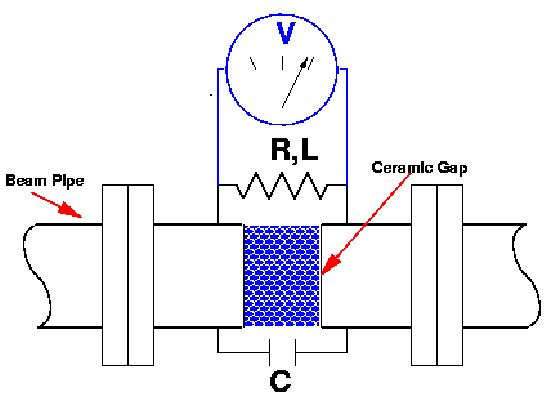
\includegraphics[width=0.75\linewidth]{./figures/wcm_schematic_cartoon}
    \caption{ 
      Shown: an insulating ceramic break in the beam pipe, which shunts
      image wall currents from the beam pipe around the toriud. Magnetic
      shielding excludes external magnetic fields.~\cite{kawallfocus2005} 
    }
    \label{fig:wcm_schematic_cartoon}
  \end{center}
\end{figure}

\begin{figure}[ht]
  \begin{center}
    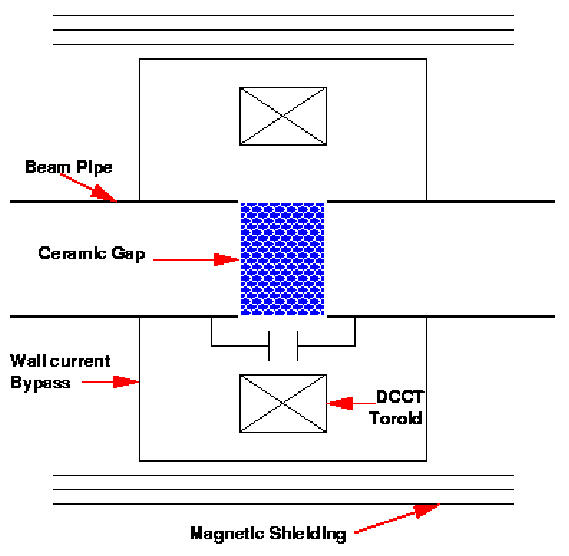
\includegraphics[width=0.75\linewidth]{./figures/dcct_schematic_cartoon}
    \caption{
      The wall current monitor uses an insulating ceramic break in the beam pipe
      similarly to the DCCT, which forces image wall currents through
      electronics which measure the current frequencies. The WCM is sensitive
      only to bunched beams, and can measure longitudianl profiles of bunches
      ~\cite{kawallfocus2005}.
    }
    \label{fig:dcct_schematic_cartoon}
  \end{center}
\end{figure}

\begin{figure}
  \centering
  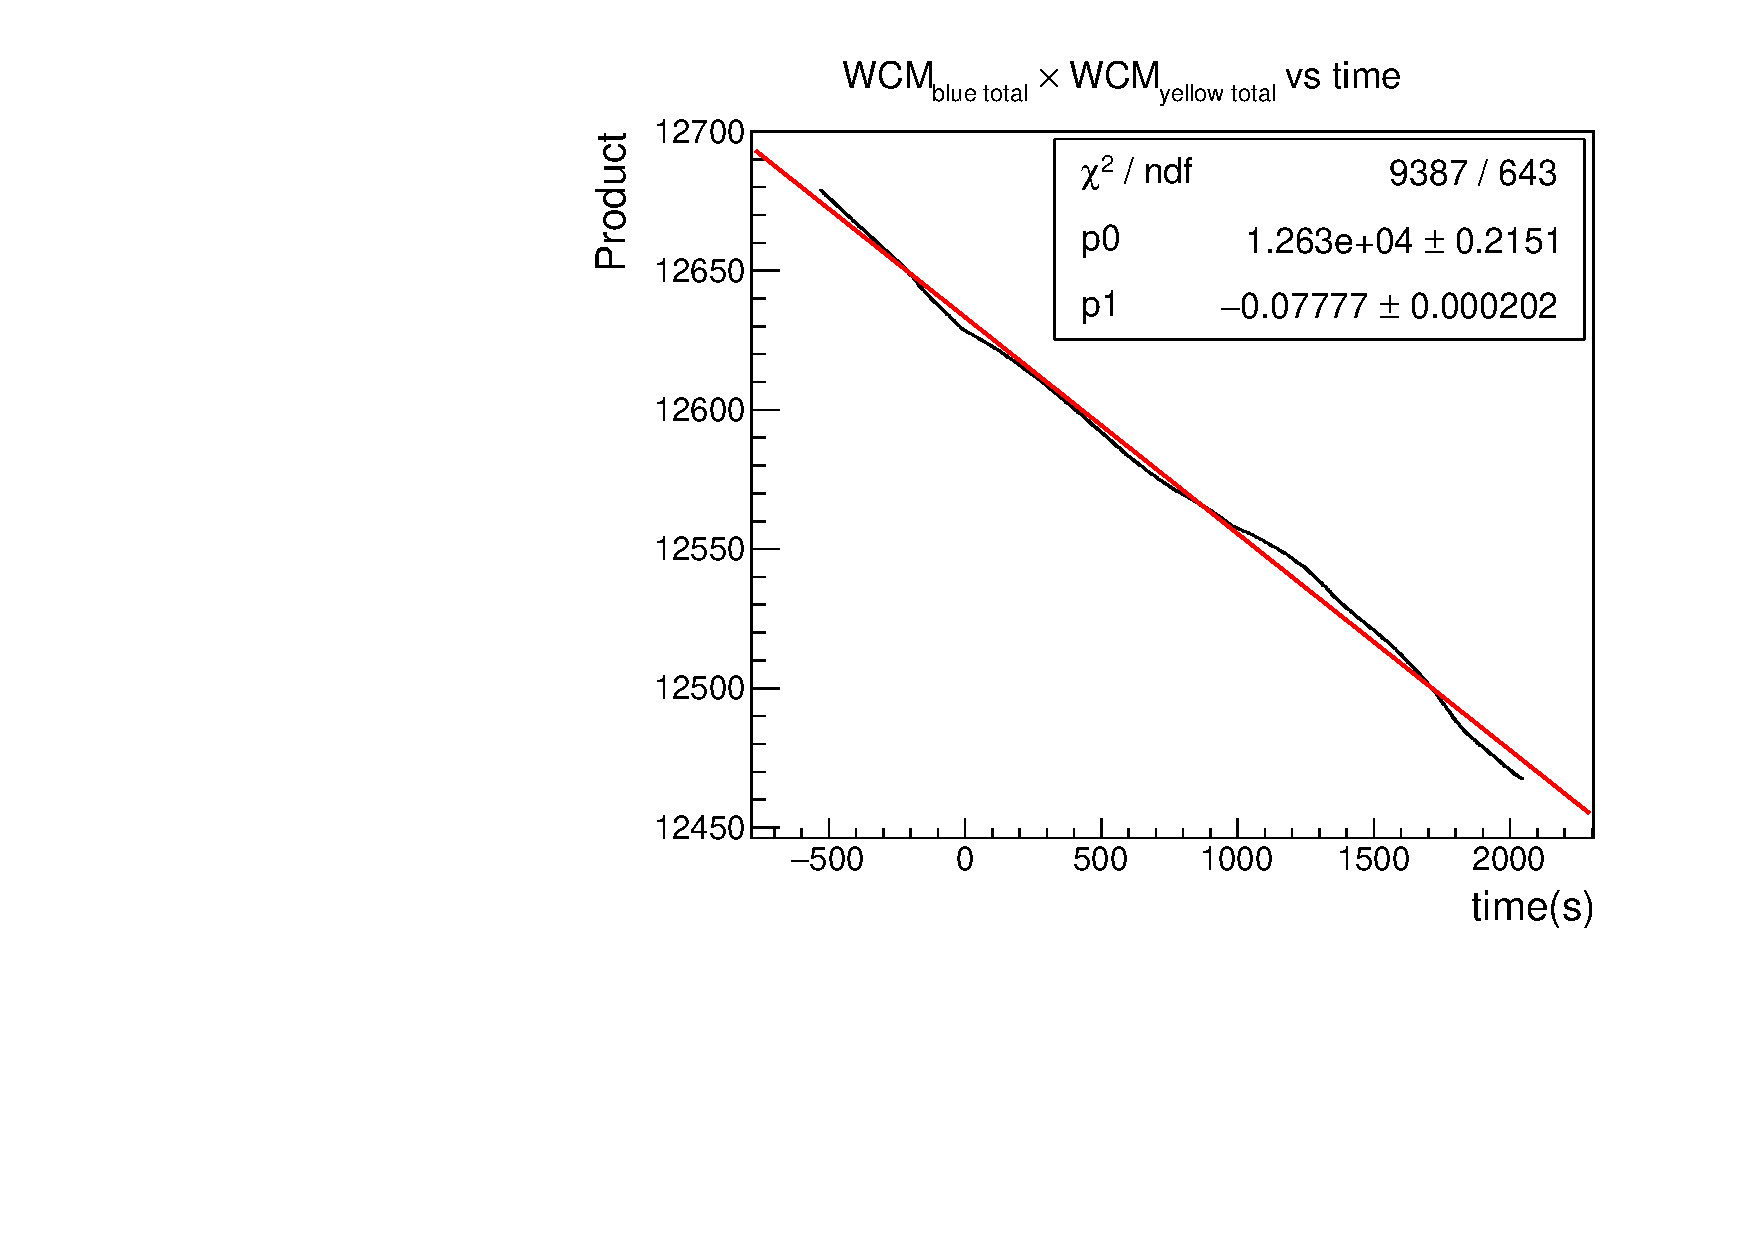
\includegraphics[width=\linewidth]{./figures/wcm_rate_loss.pdf}
  \caption{
    rate loss
  }
  \label{fig:wcm_rate_loss}
\end{figure}

\begin{figure}
  \centering
  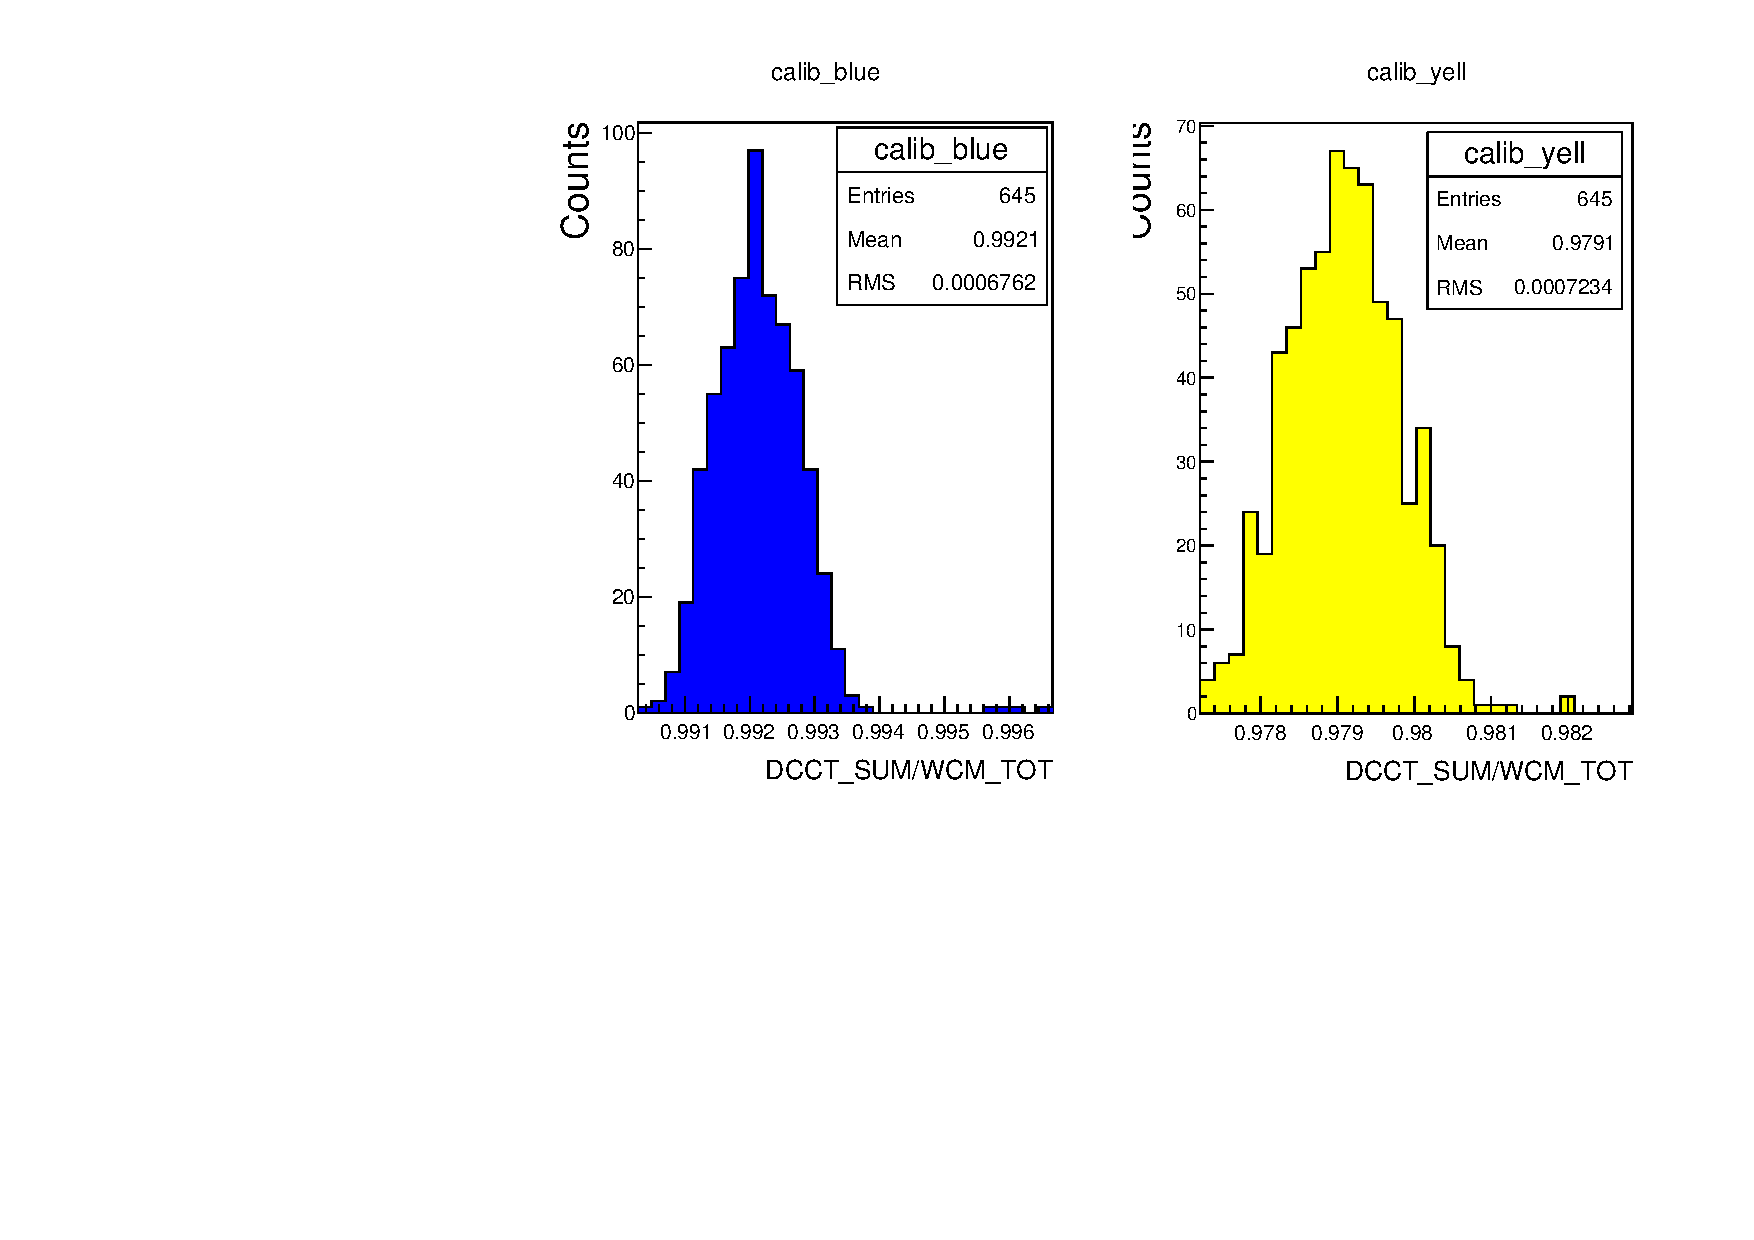
\includegraphics[width=\linewidth]{./figures/wcm_calibration_example.pdf}
  \caption{
    Left: distribution of the calibration constant for the WCM population, blue
    beam. Right: distribution of the calibration constant for the WCM
    population, yellow beam.
  }
  \label{fig:wcm_calibration}
\end{figure}

\begin{figure}
  \centering
  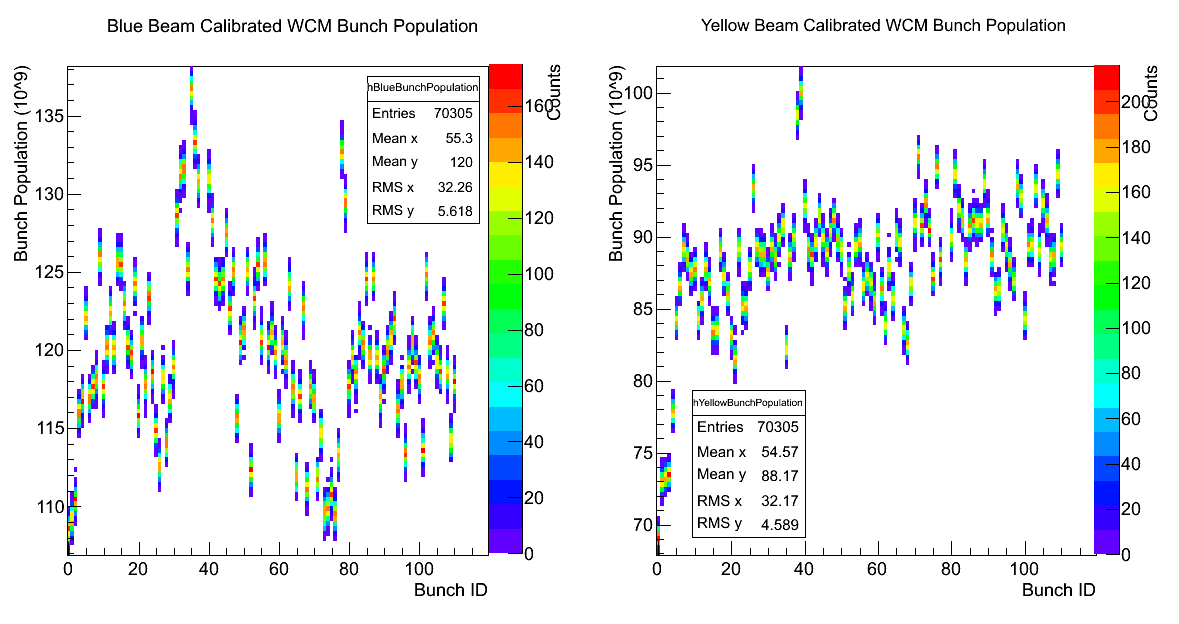
\includegraphics[width=\linewidth]{./figures/359711_bunch_population.png}
  \caption{
    Distribution of WCM population, corrected by DCCT for each bunch for an
    example run. Left: blue beam. Right: yellow beam. For both figures, the
    horizontal axis represents the bunch number.
  }
  \label{fig:bunch_population_example}
\end{figure}

\edithere{}
TODO
\begin{itemize}
    \item discuss beam population extraction
    \item discuss calibration of WCM data with DCCT data.
\end{itemize}
